\documentclass[9pt,twocolumn,twoside,lineno]{pnas-new}
% Use the lineno option to display guide line numbers if required.

\makeatletter
\newcommand*{\addFileDependency}[1]{% argument=file name and extension
  \typeout{(#1)}
  \@addtofilelist{#1}
  \IfFileExists{#1}{}{\typeout{No file #1.}}
}
\makeatother
\newcommand*{\myexternaldocument}[1]{%
    \externaldocument{#1}%
    \addFileDependency{#1.tex}%
    \addFileDependency{#1.aux}%
}
\usepackage{xr}
\myexternaldocument{manuscript/text_supporting}

\usepackage{todonotes}
\usepackage{biblatex}
\addbibresource{references}

\newcommand\focalcountry{CHE}
\newcommand\mindate{01. Jan. 2020}
\newcommand\maxdate{01. Dec. 2020}
\newcommand\maxmissing{2903}
\newcommand\minlength{27000}
\newcommand\maxsamplingfraction{0.05}
\newcommand\subsamplebycanton{TRUE}
\newcommand\travelcontextscalefactor{0}
\newcommand\similaritycontextscalefactor{2}
\newcommand\traveldataweights{1,1,1}
\newcommand\whichtrees{\.*}
\newcommand\pickchainsunderothercriteria{TRUE}
\newcommand\ntrees{-1}
\newcommand\smoothconfcases{FALSE}
\newcommand\outgroupgisaidepiisls{EPI\_ISL\_406798}
\newcommand\uniquecontextonly{FALSE}
\newcommand\maskfromstart{100}
\newcommand\maskfromend{50}

\newcommand\nchainsmin{746}
\newcommand\nchainsmax{2995}
\newcommand\minlargestchainsper{23}
\newcommand\maxlargestchainsper{14}
\newcommand\nspanningchainsmin{}
\newcommand\nspanningchainsmax{}

\newcommand\nfocalsamples{5520}
\newcommand\nsimcontext{11009}
\newcommand\ntravelcontext{0}
\newcommand\meanweeklysamplingpercent{NaN}
\newcommand\minweeklysamplingpercent{NaN}
\newcommand\maxweeklysamplingpercent{NaN}
\newcommand\overallsamplingpercent{1.4}


\templatetype{pnasresearcharticle} % Choose template 

\title{SARS-CoV-2 Genome surveillance in Switzerland: Can we quantify the effects of policy?}

% Use letters for affiliations, numbers to show equal authorship (if applicable) and to indicate the corresponding author
\author[a,c,1]{Author One}
\author[b,1,2]{Author Two} 
\author[a]{Author Three}

\affil[a]{Affiliation One}
\affil[b]{Affiliation Two}
\affil[c]{Affiliation Three}

% Please give the surname of the lead author for the running footer
\leadauthor{Lead author last name} 

% Please add a significance statement to explain the relevance of your work
\significancestatement{Authors must submit a 120-word maximum statement about the significance of their research paper written at a level understandable to an undergraduate educated scientist outside their field of speciality. The primary goal of the significance statement is to explain the relevance of the work in broad context to a broad readership. The significance statement appears in the paper itself and is required for all research papers.}

% Please include corresponding author, author contribution and author declaration information
\authorcontributions{Please provide details of author contributions here.}
\authordeclaration{Please declare any competing interests here.}
\equalauthors{\textsuperscript{1}A.O.(Author One) contributed equally to this work with A.T. (Author Two) (remove if not applicable).}
\correspondingauthor{\textsuperscript{2}To whom correspondence should be addressed. E-mail: author.two\@email.com}

% At least three keywords are required at submission. Please provide three to five keywords, separated by the pipe symbol.
\keywords{Keyword 1 $|$ Keyword 2 $|$ Keyword 3 $|$ ...} 

\begin{abstract}
% Please provide an abstract of no more than 250 words in a single paragraph. Abstracts should explain to the general reader the major contributions of the article. References in the abstract must be cited in full within the abstract itself and cited in the text.
Are the effects of policies designed to prevent and contain SARS-CoV-2 introductions evident in genomic surveillance data? Here we use SARS-CoV-2 genome sequences from approximately \overallsamplingpercent\% of all confirmed cases in Switzerland from the first case on 25. Feb. through \maxdate\ to identify local transmission chains and quantify their spread in Switzerland. We first performed a large-scale phylogenetic analysis to characterize the dynamics of virus introductions into Switzerland. We then performed a phylodynamic analysis to quantify transmission chain spread in Switzerland and test whether Switzerland’s contact tracing program was able to slow the spread of introduced lineages once local cases were identified. These analyses aim to help us understand the importance of international travel towards a national epidemic, an increasingly relevant topic as global vaccination campaigns continue at an uneven pace and new variants of concern spread internationally.
\end{abstract}

\dates{This manuscript was compiled on \today}
\doi{\url{www.pnas.org/cgi/doi/10.1073/pnas.XXXXXXXXXX}}

\begin{document}

\maketitle
\thispagestyle{firststyle}
\ifthenelse{\boolean{shortarticle}}{\ifthenelse{\boolean{singlecolumn}}{\abscontentformatted}{\abscontent}}{}

% \subsection*{Author Affiliations}

% Include department, institution, and complete address, with the ZIP/postal code, for each author. Use lower case letters to match authors with institutions, as shown in the example. PNAS strongly encourages authors to supply an \href{https://orcid.org/}{ORCID identifier} for each author. Individual authors must link their ORCID account to their PNAS account at \href{http://www.pnascentral.org/}{www.pnascentral.org}. For proper authentication, authors must provide their ORCID at submission and are not permitted to add ORCIDs on proofs.

\section{Introduction}
% If your first paragraph (i.e. with the \dropcap) contains a list environment (quote, quotation, theorem, definition, enumerate, itemize...), the line after the list may have some extra indentation. If this is the case, add \parshape=0 to the end of the list environment.
% \dropcap{T}his PNAS journal template is provided to help you write your work in the correct journal format. Instructions for use are provided below. 

% Claim importance
\dropcap{T}o stem a national epidemic, public health policies must prevent or break local transmission chains. However, contact tracing data to reconstruct and investigate transmission chains - and the effect of policies on their spread - is difficult to collect and sensitive. Alternatively, pathogen genomes can provide information to estimate introduction and transmission dynamics. In particular, fast-mutating RNA viruses like SARS-CoV-2 accumulate mutations on the same time-scale as they are transmitted. These mutations allow estimation of a viral phylogeny, which is an approximation of the epidemic transmission tree. Therefore, pathogen genomes can be used to estimate past transmission dynamics, given a suitably fast-mutating virus and representative genome sampling.

SARS-CoV-2 genome data have been extensively used to characterize and quantify transmission dynamics for regional COVID-19 epidemics. Phylogenetic approaches are generally used to identify events like introductions, super-spreading, and transmission chains from SARS-CoV-2 phylogenies, e.g. \cite{Lu2020, Eden2020, OudeMunnink2020, Bluhm2020}. Going one step further, more complex phylodynamic approaches fit a demographic model to the phylogeny, where branching times are explained by population demographic parameters \cite{Grenfell2004}. Thus, the phylodynamic approach enables estimation of population-wide dynamics, while the phylogenetic approach is specific to the analyzed samples.

Importantly, both phylogenetic and phylodynamic approaches can help assess public health policy effects on epidemic spread. For instance, \cite{Mallon2020, duPlessis2021} showed that in the first-wave of the Irish and English SARS-CoV-2 epidemics, national lock-downs led to major reductions in lineage diversity and size. Using phylodynamic methods, \cite{Miller2020, Geoghegan2020a, Muller2020a} found that the reproductive number of SARS-CoV-2 decreased after the introduction of non-pharmaceutical interventions (NPIs) and/or reductions in mobility indices in Israel, New Zealand, and Washington State, USA, respectively. Finally, \cite{Ragonnet-Cronin2021} used genome and line-list data across many regions to uncover a correlation between the time difference from  (phylogenetically-estimated) epidemic start to strongest regional NPI and the number of regional deaths. However, the utility of genome data for evaluating specific policy effects at the regional level is still largely unexplored.

% Indicate a gap
% Right now not clear why we don't follow the approaches of either UK or Israel/NZ/WA
Parametric inference using genome sequence data is complicated for several reasons. One problem is sampling bias; genome sequencing efforts can be highly variable across regions and through time, so genome samples may not be a representative, random sample from the studied epidemic  \cite{Villabona-Arenas2020, DeMaio2015}. A second problem is phylogenetic uncertainty; if viral diversity in the studied epidemic is either too low or too high, there is little information for reconstructing phylogenetic releationships  \cite{Villabona-Arenas2020}. In either case, phylogenetic inferences may be misleading or overly confident. Phylodynamic models can account for sampling bias by fitting  time-varying sampling and transmission rates to structured populations and for phylogenetic uncertainty by integrating over many possible phylogenies \cite{Scire2020b}. However, such models are generally too computationally complex to fit to thousands of genomes. 
% In the absence of strong prior information, these models are also too richly parameterized to be identifiable \cite{Louca2021FundamentalEpidemiology}.

% State that our paper fills the gap
In this work, we use thousands of SARS-CoV-2 genomes collected across Switzerland since the epidemic start to characterize aspects of the Swiss SARS-CoV-2 epidemic that cannot be accessed from line-list data alone. Namely, we aim to quantify introductions, transmission chains, and evidence for a slow in transmission upon transmission chain detection. To do this, we carefully combine phylogenetic and phylodynamic approaches in a two-step analysis that allows us to analyze thousands of genomes in $<$ 12 hours while limiting sampling bias and accounting for phylogenetic uncertainty. In the first step, we construct an approximate maximum-likelihood phylogeny for each SARS-CoV-2 Pango lineage and identify Swiss transmission chains within these lineages. In the second step, we jointly infer time-varying transmission dynamics of the Swiss epidemic, conditioned on these transmission chains, using a Bayesian phylodynamic framework. In each step, we condition on monophyletic partitions of the sample set, an approach inspired by previous work by \cite{DuPlessis} and \cite{Muller2020}. This ensures the computational feasibility of our analysis. To limit sampling biases, we sub-sample genomes from the Swiss nation-wide genome surveillance program to be as spatio-temporally representative of the Swiss epidemic as possible. To incorporate uncertainty in phylogenetic estimates for introductions and transmission chains, we report upper- and lower-bound estimates generated under two extreme resolutions of polytomies. Bayesian phylodynamic estimates for transmission dynamics naturally incorporate phylogenetic uncertainty within each transmission chain by integrating over many plausible phylogenies.

% Intro our results
Based on our phylogenetic analysis, we show the dynamics of virus introductions into Switzerland in relation to border policy changes. Then, based on our phylodynamic analysis, we quantify transmission chain spread in Switzerland and test whether Switzerland’s contact tracing program helped slow transmission.

\section{Results}

\subsection{Introductions composing the Swiss epidemic}

We analyzed \nfocalsamples\ SARS-CoV-2 genomes collected in Switzerland, representing the Swiss epidemic from the first detected case on 25. Feb. through 31. Dec. 2020 \ref{fig:downsampling_representativeness}. We estimate these samples came from between \nchainsmin\ and \nchainsmax\ independent introductions into Switzerland. The resulting Swiss transmission chains are roughly power law-distributed in size, with the 10 largest chains accounting for \maxlargestchainsper\ to \minlargestchainsper \% of genome samples \ref{fig:chain_size_dist}. From a down-sampling analysis, we see that we do not reach saturation - if we were to include more genomes, we would likely identify more introductions \ref{fig:sensitivity_downsampling}. 

% section on geographic distribution of chains

% Validation of the identified introductions is difficult without detailed contact tracing data. However, we can reference a small subset of samples for which we have recorded foreign exposure locations from the Swiss Federal Office for Public Health. We expect these samples to be singletons or the index case(s) of  transmission chains. Given the largest plausible introductions, \ncinongruentexposurechainsmin\ out of \nexposurechainsmin\ introductions with at least one sample exposed abroad have exposures from multiple countries (so, incongruous with introductions having one or a few index cases returning from the same country). Given the smallest plausible introductions, this fraction drops to \ncinongruentexposurechainsmax\ out of \nexposurechainsmax. The median rank of  exposed samples is  \rankexpsamplemin nd in the largest plausible transmission chains and \rankexpsamplemax st in the smallest. We note that these validation metrics are flawed, since each genome being a separate introduction - quite unrealistic - results in perfect agreement. However, the results give us some indication that the smallest plausible introductions are more realistic.

% International comparison: UK chain sizes have power-law decay w/ alpha = 0.79 for chains 2 <= x <= 50, 1.26 for chains > 50. 
% Similar to Louis, I see chain sizes as power-law distributed, with a change in scale factor at ~ chain size 50. 
% The scaling factors I estimate are higher than his though (~1.2 for <= 50 and ~1.4 for >50). So, our Swiss chain sizes decay more sharply (fewer larger chains) than his UK chains.

\subsection{Resulting Swiss transmission chains}
We show the number and longevity of transmission chains by the month they were fist sampled in \ref{fig:chain-longevity}. From \ref{fig:chain-longevity} we see that the number and longevity of transmission chains is affected by phylogenetic uncertainty. A small number of transmission chains - between \nspanningchainsmax\ and \nspanningchainsmin\ - appear to have persisted in Switzerland from the start of the epidemic in Mar. 2020 until the end of the sampling period in Dec. 2020. Fewer new transmission chains were sampled in the months following the partial closure of Swiss borders bewteen 25. Mar. and 14. Jun. 2020. 
\begin{figure}[tbhp]
\centering
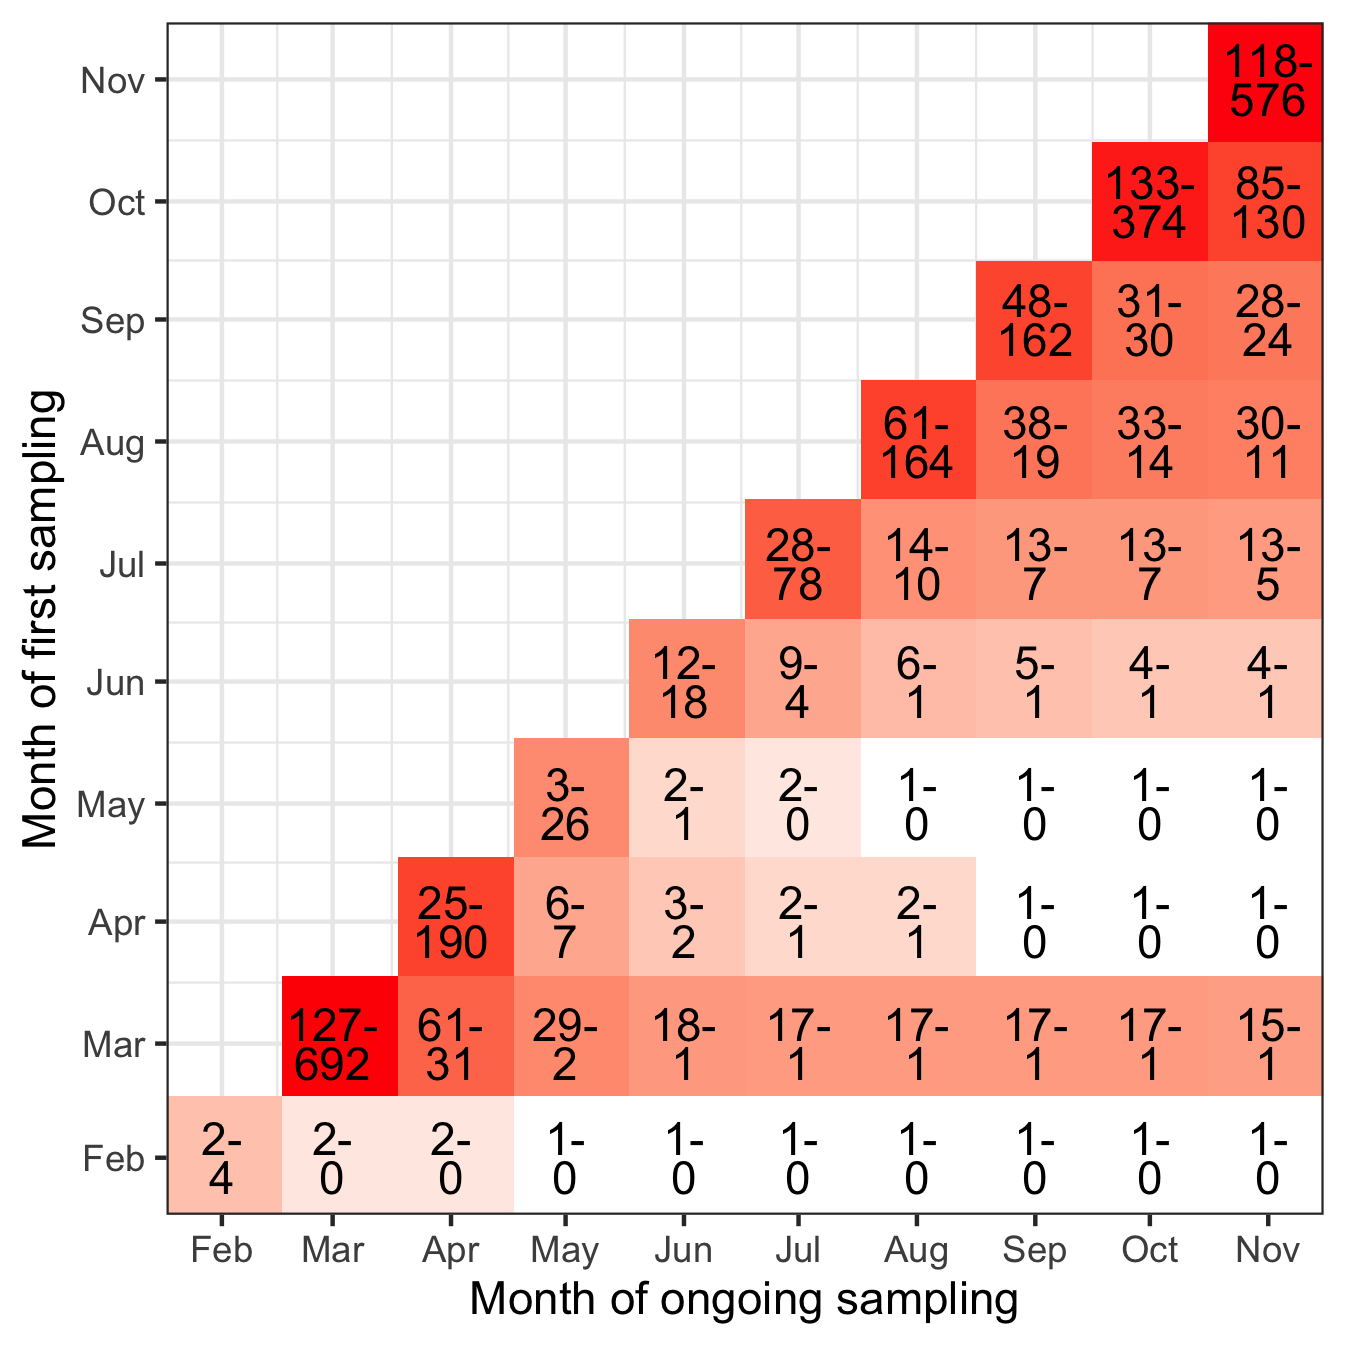
\includegraphics[width=.8\linewidth]{figures/chain_longevity_matrix.png}
\caption{Number of ongoing Swiss transmission chains by the month they were fist sampled. Estimate ranges are between analyses assuming the minimum and maximum plausible number of transmission chains in total. Darker red squares have a higher number of ongoing transmission chains, averaged over the two analyses.}
\label{fig:chain-longevity}
\end{figure}

\subsection{Time-varying transmission dynamics within Switzerland}
\begin{figure}[tbhp]
\centering
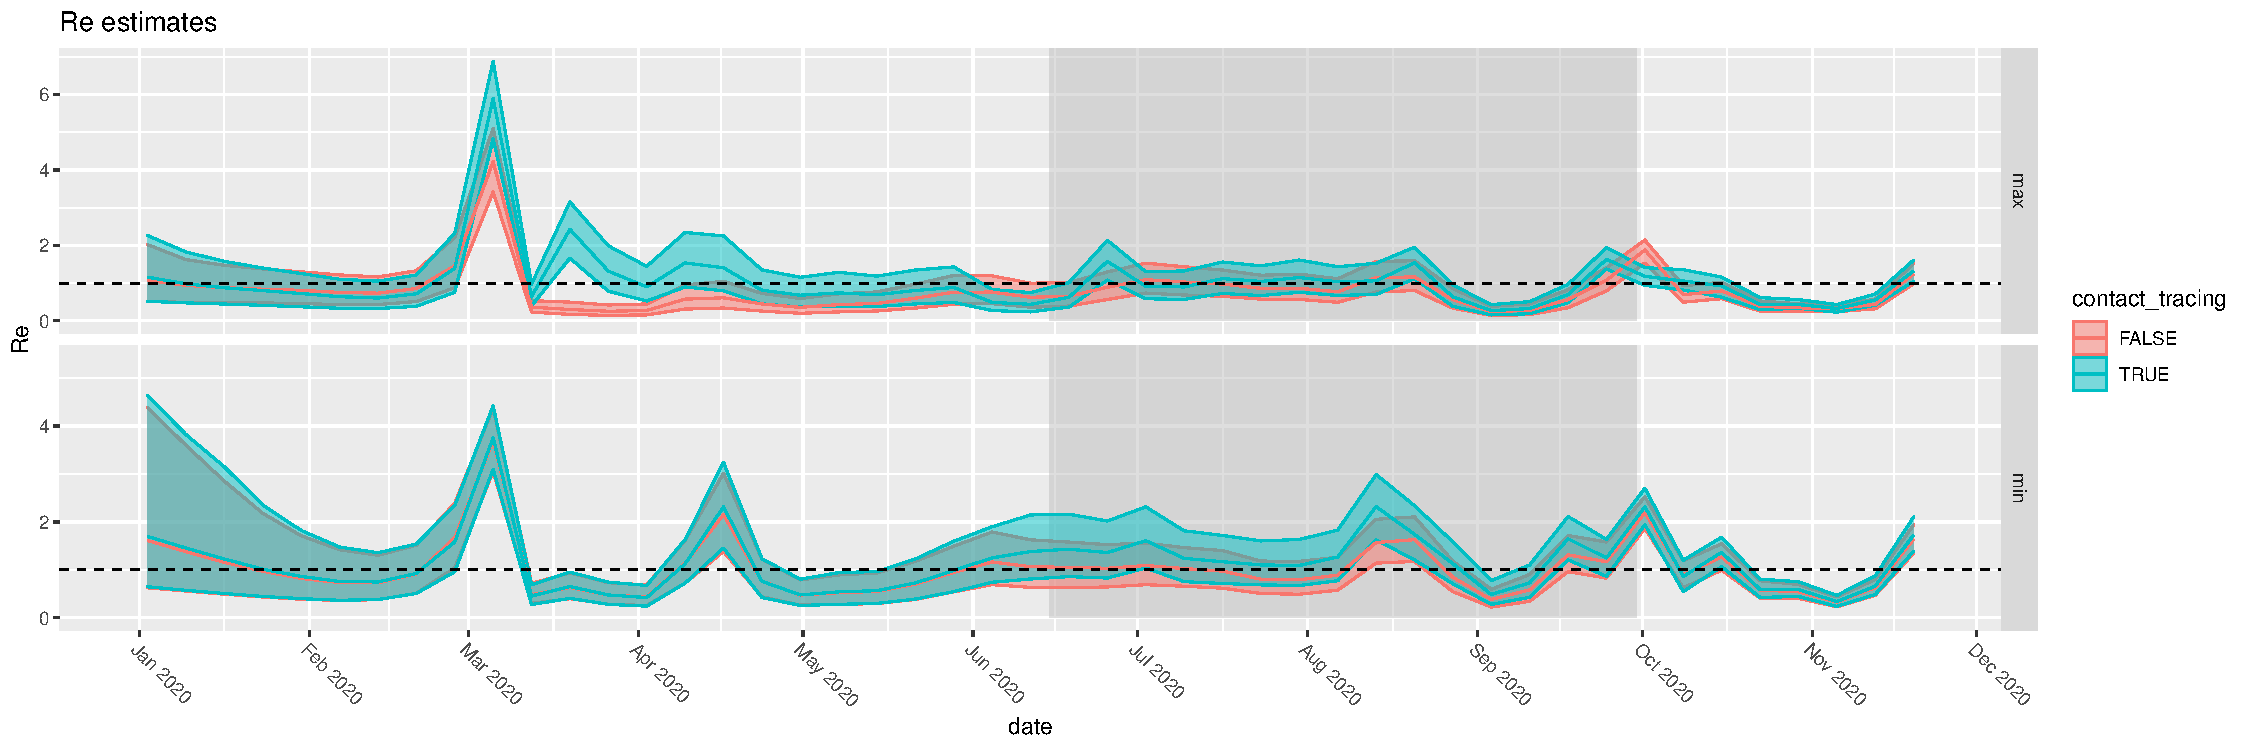
\includegraphics[width=.8\linewidth]{figures/Re_noSampUB.pdf}
\caption{Effective reproductive number estimated under the largest and smallest plausible introductions scenarios in analyses with and without a ``contact tracing'' scale factor.}  
\label{fig:scale-factor}
\end{figure}

\subsection{Testing for slowed transmission upon transmission chain detection}

\begin{figure}[tbhp]
\centering
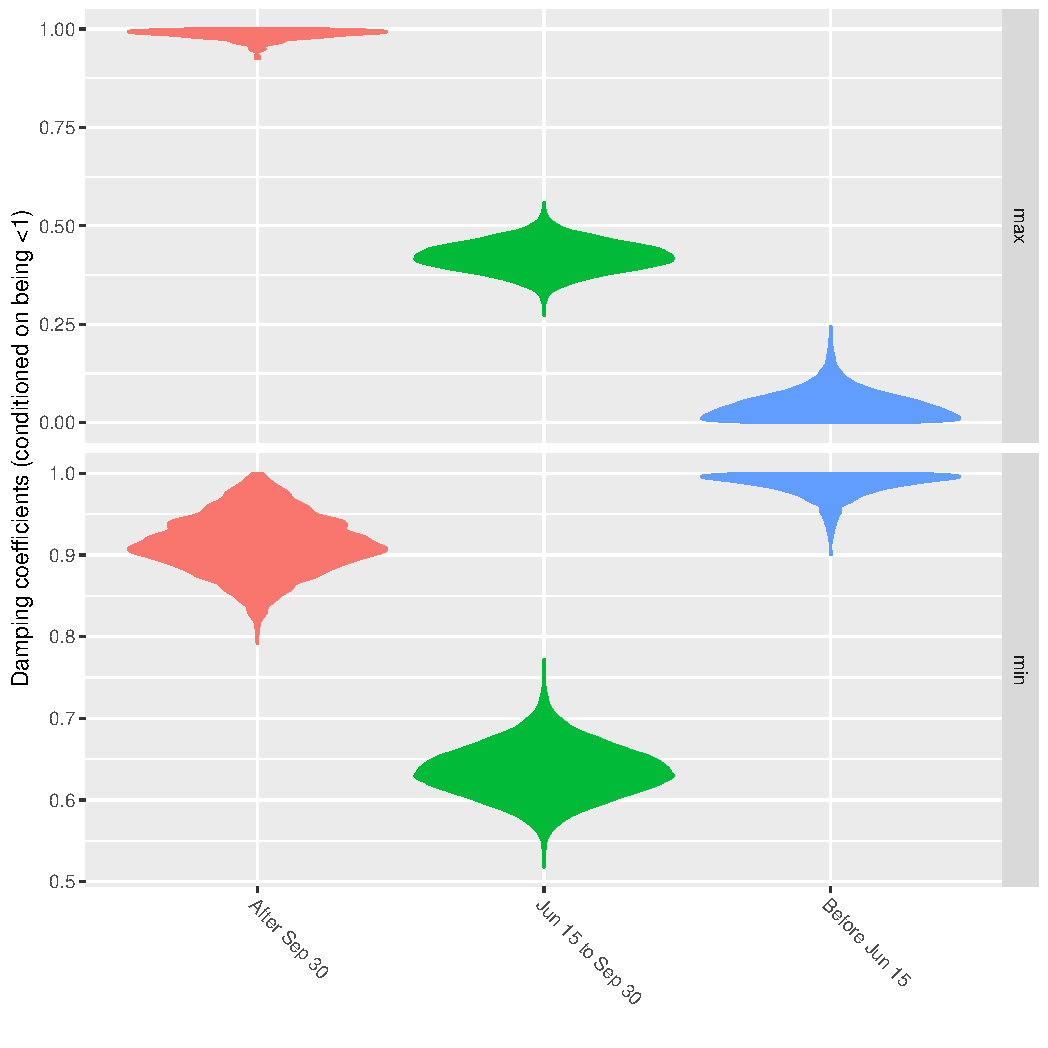
\includegraphics[width=.8\linewidth]{figures/CT_conditionedDamping_noSampUB.pdf}
\caption{``Contact tracing'' scale factor estimated in three different time periods under the largest and smallest plausible introductions scenarios.}  
\label{fig:scale-factor}
\end{figure}

% \begin{itemize}
%     \item Spike and slab prior for Re multiplier
%     \item Bounded time-frame for Re multiplier
%     \item Sampling proportion upper bound 0.01 instead of 0.1 - Tim will rerun
%     \item Prior on cluster origins is not unique to each cluster, it's a big lognormal blob throughout 2020 - Tim will switch to unif(Jan 1 - Dec 31) so that our prior assumption is that the rate of introductions is constant from when the pandemic started spreading internationally until end of sampling period
%     \item How indep are Re estimates from phylo when I select seqs based on conf case \#s? - Tanja's not concerned, the genomes can still tell us what they tell us within what we already know from cases
%     \item 50\% prior y/n need Re factor, if y then unif(0, 1) on the factor 
%     \item Tim puts independent spike & slab priors in spring, summer, and fall and infers three Re reduction factors so we can see if Summer is really different
%     \item Remember Re plot is now background Re (without contact tracing) and no longer the actual average Re
% \end{itemize}

\section{Discussion}
\begin{itemize}
    \item Estimates on introductions and transmission chains are sensitive to phylogenetic uncertainty
    \begin{itemize}
        \item TODO: How does this compare to other studies?
        \item Recommend caution in trying to show who-infected-who when transmission timescale faster than mutational timescale
    \end{itemize}
    \item We treat the time-varying sampling proportion as a fitting parameter
    \begin{itemize}
        \item 
    \end{itemize}
    \item Contact tracing at the national level isn't as effective for new introductions.
    \begin{itemize}
        \item We find robust signal for decrease in transmission after chain detection in Summer 2020 compared to Spring 2020. Fall 2020 inference is not robust to phylogenetic uncertainty. 
        \item This slow correlates with the approximate start to contact tracing efforts, but an alternate explanation could be that sampled transmission chains originate in early super-spreading events.
    \end{itemize}
\end{itemize}
% MAJOR QUESTION: was the summer epidemic growing in size due to travel (ie import of strains which seeded local transmission chains)?
% Contact tracing factor could also be catching superspreading events that found transmission chains

\section{Acknowledgments}



% \subsection*{Submitting Manuscripts}

% All authors must submit their articles at \href{http://www.pnascentral.org/cgi-bin/main.plex}{PNAScentral}. If you are using Overleaf to write your article, you can use the ``Submit to PNAS'' option in the top bar of the editor window. 

% \subsection*{Format}

% Many authors find it useful to organize their manuscripts with the following order of sections;  title, author line and affiliations, keywords, abstract, significance statement, introduction, results, discussion, materials and methods, acknowledgments, and references. Other orders and headings are permitted.

% \subsection*{Manuscript Length}

% A standard 6-page article is approximately 4,000 words, 50 references, and 4 medium-size graphical elements (i.e., figures and tables). The preferred length of articles remains at 6 pages, but PNAS will allow articles up to a maximum of 12 pages.

\subsection*{References}
\printbibliography

% References should be cited in numerical order as they appear in text; this will be done automatically via bibtex, e.g. \cite{belkin2002using} and \cite{berard1994embedding,coifman2005geometric}. All references cited in the main text should be included in the main manuscript file.

% \subsection*{Data Archival}

% PNAS must be able to archive the data essential to a published article. Where such archiving is not possible, deposition of data in public databases, such as GenBank, ArrayExpress, Protein Data Bank, Unidata, and others outlined in the \href{https://www.pnas.org/page/authors/journal-policies#xi}{Information for Authors}, is acceptable.

% \subsection*{Language-Editing Services}
% Prior to submission, authors who believe their manuscripts would benefit from professional editing are encouraged to use a language-editing service (see list at www.pnas.org/page/authors/language-editing). PNAS does not take responsibility for or endorse these services, and their use has no bearing on acceptance of a manuscript for publication. 

% \begin{figure}%[tbhp]
% \centering
% 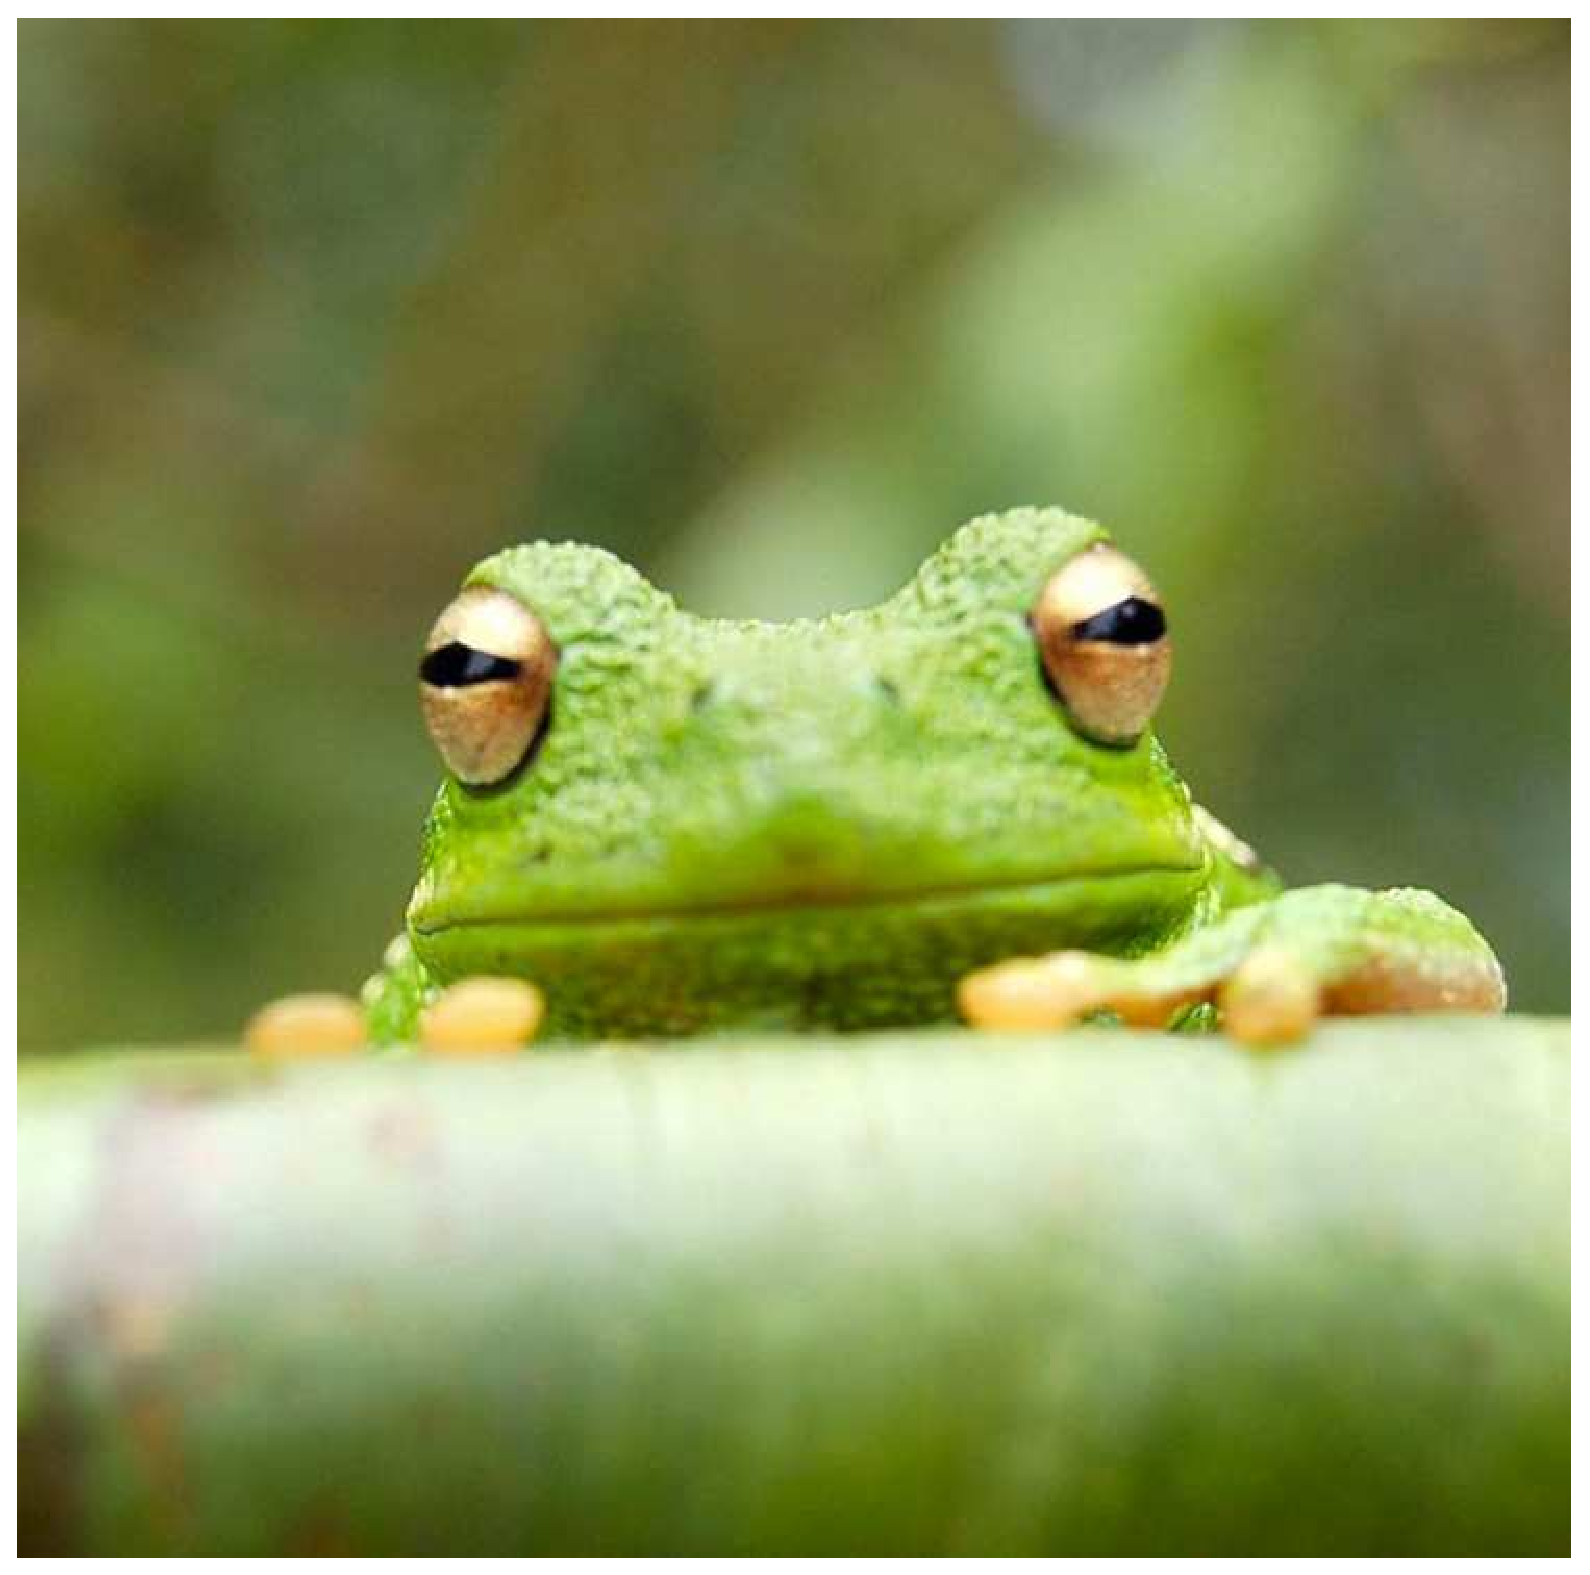
\includegraphics[width=.8\linewidth]{frog}
% \caption{Placeholder image of a frog with a long example legend to show justification setting.}
% \label{fig:frog}
% \end{figure}


% \begin{SCfigure*}[\sidecaptionrelwidth][t]
% \centering
% 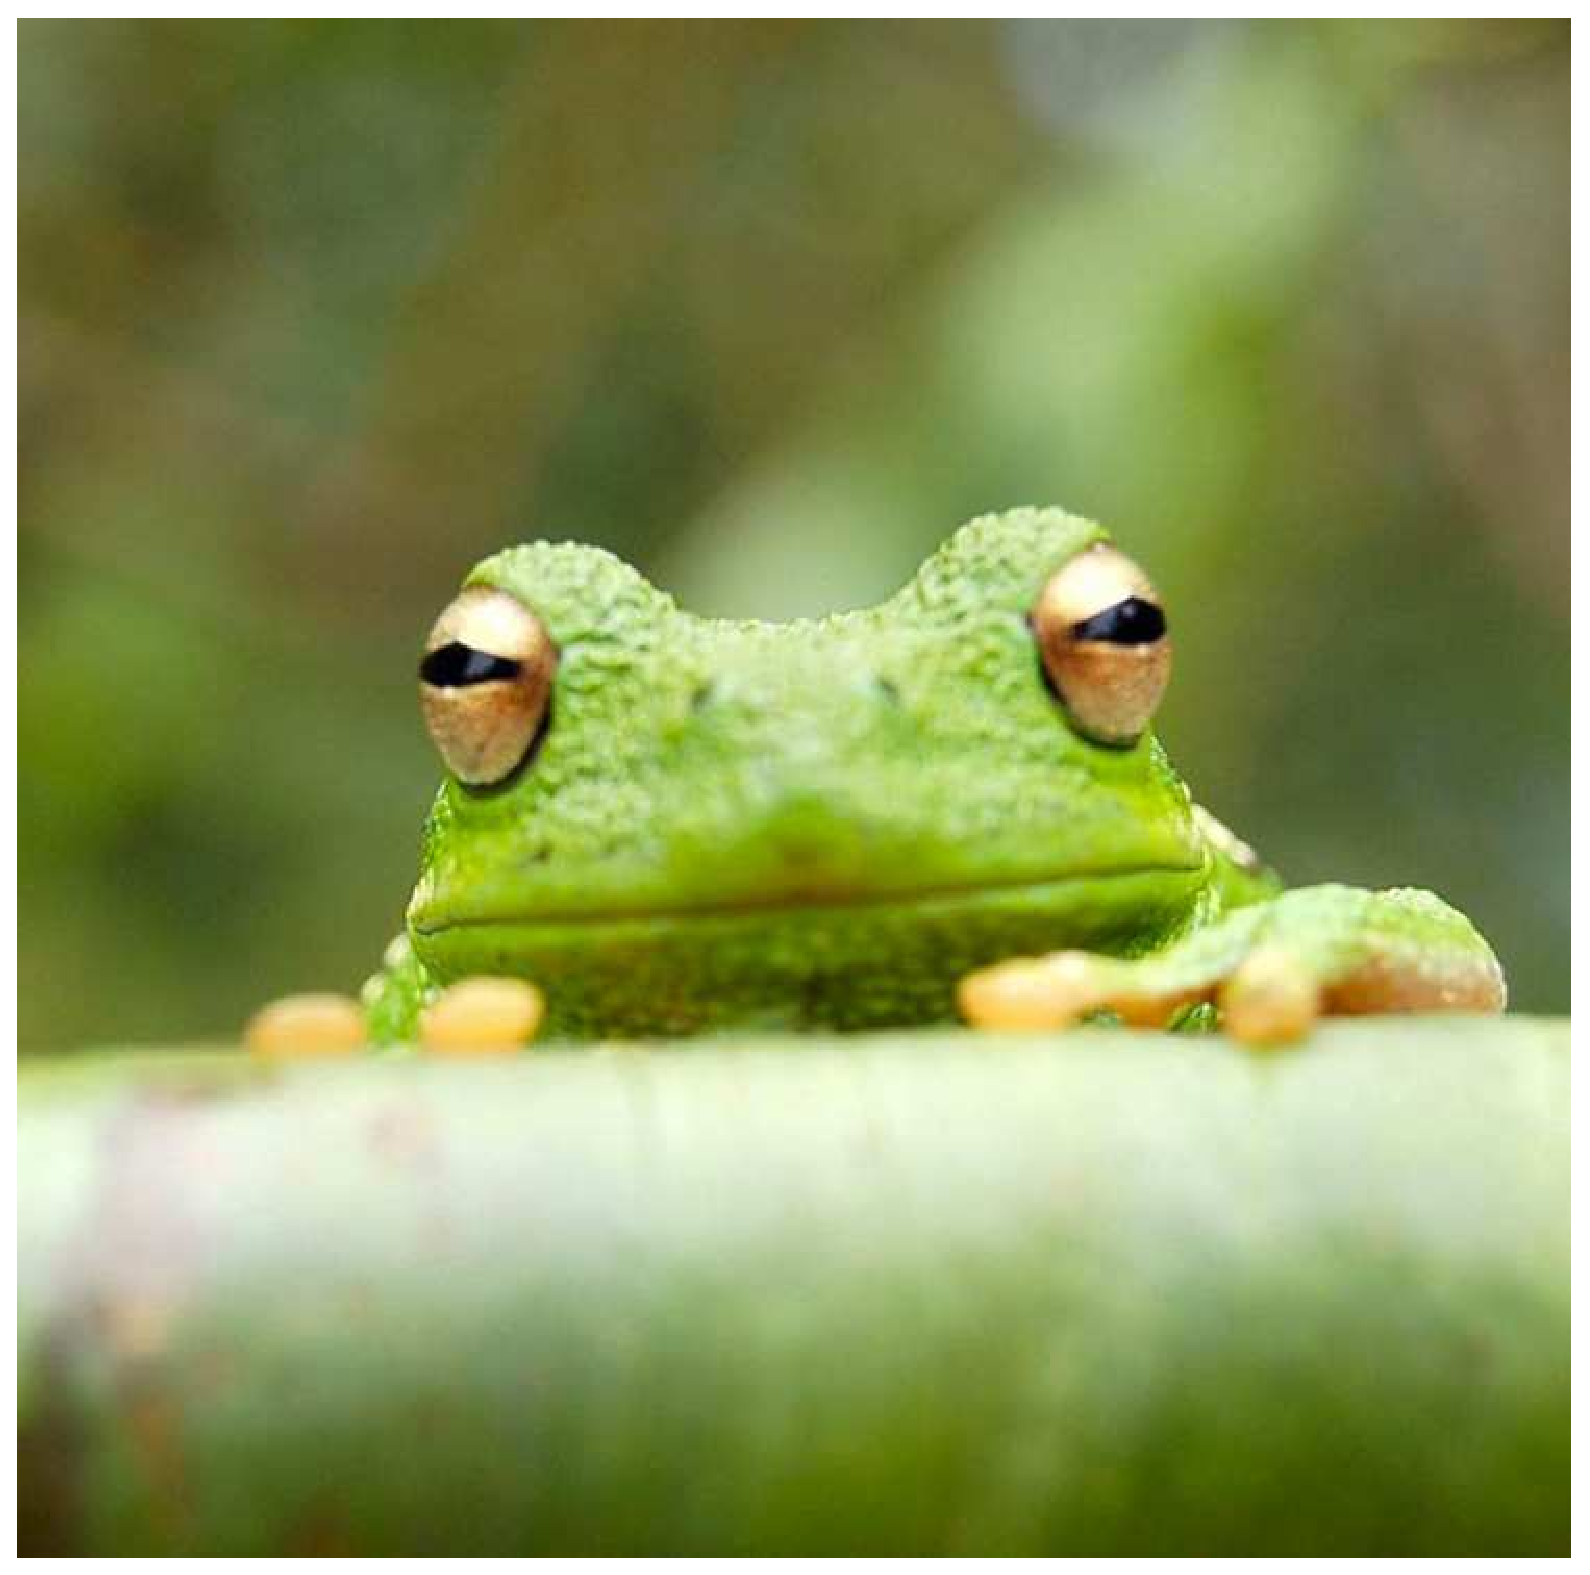
\includegraphics[width=11.4cm,height=11.4cm]{frog}
% \caption{This legend would be placed at the side of the figure, rather than below it.}\label{fig:side}
% \end{SCfigure*}

% \subsection*{Digital Figures}

% EPS, high-resolution PDF, and PowerPoint are preferred formats for figures that will be used in the main manuscript. Authors may submit PRC or U3D files for 3D images; these must be accompanied by 2D representations in TIFF, EPS, or high-resolution PDF format. Color images must be in RGB (red, green, blue) mode. Include the font files for any text.

% Images must be provided at final size, preferably 1 column width (8.7cm). Figures wider than 1 column should be sized to 11.4cm or 17.8cm wide. Numbers, letters, and symbols should be no smaller than 6 points (2mm) and no larger than 12 points (6mm) after reduction and must be consistent. 

% Figures and tables should be labelled and referenced in the standard way using the \verb|\label{}| and \verb|\ref{}| commands.

% Figure \ref{fig:frog} shows an example of how to insert a column-wide figure. To insert a figure wider than one column, please use the \verb|\begin{figure*}...\end{figure*}| environment. Figures wider than one column should be sized to 11.4 cm or 17.8 cm wide. Use \verb|\begin{SCfigure*}...\end{SCfigure*}| for a wide figure with side legends.

% \subsection*{Tables}
% Tables should be included in the main manuscript file and should not be uploaded separately.

% \subsection*{Single column equations}

% Authors may use 1- or 2-column equations in their article, according to their preference.

% To allow an equation to span both columns, use the \verb|\begin{figure*}...\end{figure*}| environment mentioned above for figures.

% Note that the use of the \verb|widetext| environment for equations is not recommended, and should not be used. 

% \begin{figure*}[bt!]
% \begin{align*}
% (x+y)^3&=(x+y)(x+y)^2\\
%       &=(x+y)(x^2+2xy+y^2) \numberthis \label{eqn:example} \\
%       &=x^3+3x^2y+3xy^3+x^3. 
% \end{align*}
% \end{figure*}


% \begin{table}%[tbhp]
% \centering
% \caption{Comparison of the fitted potential energy surfaces and ab initio benchmark electronic energy calculations}
% \begin{tabular}{lrrr}
% Species & CBS & CV & G3 \\
% \midrule
% 1. Acetaldehyde & 0.0 & 0.0 & 0.0 \\
% 2. Vinyl alcohol & 9.1 & 9.6 & 13.5 \\
% 3. Hydroxyethylidene & 50.8 & 51.2 & 54.0\\
% \bottomrule
% \end{tabular}

% \addtabletext{nomenclature for the TSs refers to the numbered species in the table.}
% \end{table}

% \subsection*{Supporting Information Appendix (SI)}

% Authors should submit SI as a single separate SI Appendix PDF file, combining all text, figures, tables, movie legends, and SI references. SI will be published as provided by the authors; it will not be edited or composed. Additional details can be found in the \href{https://www.pnas.org/authors/submitting-your-manuscript#manuscript-formatting-guidelines}{PNAS Author Center}. The PNAS Overleaf SI template can be found \href{https://www.overleaf.com/latex/templates/pnas-template-for-supplementary-information/wqfsfqwyjtsd}{here}. Refer to the SI Appendix in the manuscript at an appropriate point in the text. Number supporting figures and tables starting with S1, S2, etc.

% Authors who place detailed materials and methods in an SI Appendix must provide sufficient detail in the main text methods to enable a reader to follow the logic of the procedures and results and also must reference the SI methods. If a paper is fundamentally a study of a new method or technique, then the methods must be described completely in the main text.

% \subsubsection*{SI Datasets} 

% Supply .xlsx, .csv, .txt, .rtf, or .pdf files. This file type will be published in raw format and will not be edited or composed.


% \subsubsection*{SI Movies}

% Supply Audio Video Interleave (avi), Quicktime (mov), Windows Media (wmv), animated GIF (gif), or MPEG files. Movie legends should be included in the SI Appendix file. All movies should be submitted at the desired reproduction size and length. Movies should be no more than 10MB in size.


% \subsubsection*{3D Figures}

% Supply a composable U3D or PRC file so that it may be edited and composed. Authors may submit a PDF file but please note it will be published in raw format and will not be edited or composed.


\matmethods{

\subsection*{Genome sequencing and quality filtering}
Most of the Swiss SARS-CoV-2 genomes analyzed until 31. Dec 2020 were generated by the Swiss SARS-CoV-2 Sequencing Consortium. Here, we briefly describe the swab-to-sequence process for these samples. RNA extracts from qPRC-positive patient naso- or oral-pharangeal swabs were provided by Viollier AG, a Swiss medical diagnostics company. RNA extraction was done with either the Abbott m2000sp or Seegene STARMag 96x4 Universal Cartridge RNA extraction kit. Extracts were then  transferred to the Genomics Facility Basel or the Functional Genomics Center Zurich for whole-genome sequencing. Both centers used the ARCTIC v3 primer scheme \cite{Quick2017, ARCTICNetwork} to generate tiled, approximately 400bp-long amplicons. Library preparation was done with the New England Biolabs (NEB) library preparation kit. Libraries were sequenced on Illumina MiSeq or NovaSeq machines, resulting in 2 x 251 base reads. Bioinformatics was done using V-pipe \cite{Posada-Cespedes2020}, including read trimming and filtering with PRINSEQ \cite{Schmieder2011}, alignment to Genbank accession MN908947 \cite{Wu2020} with bwa \cite{Li2009}, and consensus base calling. For consensus base calling, positions with $<$5x coverage are masked with ``N'', positions with $>$5\% and $>$2 reads supporting a minor base are called with IUPAC ambiguity codes, and positions with $>$50\% reads supporting a deletion are called with ``-''. We rejected samples with $<$20,000 non-N bases. The consensus sequences we generated have been made publicly available on both GISAID (submitting lab: Department of Biosystems Science and Engineering, ETH Zürich) and ENA (study: PRJEB38472).

We supplemented our Swiss data with other Swiss sequences and foreign sequences available via GISAID (accessed 31. May 2021). From the full set of sequences available on GISAID, we removed from consideration non-human samples, samples $<$ 27000 bases long, and samples flagged by the Nextclade tool \cite{Aksamentov} for one of the following reasons: suspiciously clustered SNPs (QC SNP clusters status metric not ``good''; $>=$ 6 mutations in 100 bases), too many private mutations (QC private mutations status metric not ``good''; $>=$ 10 mutations from the nearest tree node), or overall bad quality (Nextclade QC overall status ``bad''). We aligned the sequences to the reference genome MN908947.3 using MAFFT \cite{katoh_mafft:_2002}. Finally, we followed the Nextstrain pipeline's recommendation to mask the first 100 and last 50 sites of the alignment \cite{Nextstraina} since the start and end of SARS-CoV-2 sequences are prone to sequencing error \cite{DeMaio2020}.

\subsection*{Sampling procedure}

From the quality-filtered alignment of GISAID sequences, we selected a focal set of sequences from Switzerland and a context set of sequences from abroad. 

% describe representativeness of Swiss dataset here too?
For the focal sequences from Switzerland, we aimed to select a spatially and temporally representative sample. Therefore, we down-sampled available sequences to \maxsamplingpercent\% of confirmed case counts in each Swiss Canton each week between \mindate\ and \maxdate. Where there were not enough sequences available from a Canton in a week, we took the maximum available sequences. To reduce the size of the alignments for phylogenetic analysis, we divided the focal Swiss set into Pango lineages \cite{Rambaut}, similar to \cite{DuPlessis2021}. Lineages composed of $>=$ 50\% Swiss sequences were aggregated into their parent lineage(s) until $<$ 50\% were Swiss. This aims to ensure that each analyzed lineage originated outside of Switzerland.

% describe nextstrain priority protocol for sim dataset
For the context sequences from abroad, we aimed to select the most genetically similar sequences to focal Swiss sequences. This set should help distinguish between SARS-CoV-2 strains unique to Switzerland (likely within-Switzerland transmission) and strains also circulating abroad (possibly recent introductions). To select this set, we applied the Nextstrain priority script \cite{Nextstrain} to rank sequences from abroad by their genetic similarity to Swiss sequences in each lineage alignment. Then, we selected \gensimscalefactor times as many most context sequences as focal Swiss sequences for each analyzed lineage. 

% describe context set estimation
% To generate the context dataset, we selected \travelcontextscalefactor\ times as many foreign genomes as Swiss genomes proportionally to monthly incidence- and travel-based estimates of SARS-CoV-2 introductions and irregardless of Pango lineage. Estimated introductions were based on case exposure locations recorded by the Swiss Federal Office for Public Health (FOPH), data on tourist arrivals at hotels published by the Swiss Federal Statistical Office (FSO), and data on the number of cross-border commuter permit holders published by the FSO. Here we aim to construct a reasonable prior estimate for monthly introductions into Switzerland and recognize that these estimates are sensitive to our subjective weighting of various data sources. Therefore, we interpret our geographic inferences in the context of these assumptions.

% Given our estimates for monthly SARS-CoV-2 introductions, we randomly selected genomes available on GISAID as of \GISAIDpulldate\ proportional to these estimates. For months without enough genomes from a country, we took extra sequences from the following month if possible and the preceding month if necessary. 

% describe sensitivity analyses here
% We applied this sub-sampling protocol three times with different random seeds. As an additional sensitivity check, we also padded the estimated introductions per country and month by 1 before determining the number of context sequences to take. Based on the padded numbers, we randomly chose another set of context sequences. In all, we analyzed three replicate context datasets and one context dataset based on padded introductions. In the main text, we discuss results based on only one of the replicate datasets; results from the other datasets are qualitatively similar (Fig. S8 – S10).

% summarize the sample set
The final dataset for analysis includes \nswissseqs\ focal sequences from Switzerland and \nsimseqs\ genetically similar context sequences from abroad.

\subsection*{Timetree generation}
We estimated the maximum likelihood phylogeny for each lineage alignment using IQ-TREE \cite{Nguyen2014} under an HKY substitution model \cite{Hasegawa1985} with empirical base frequencies and 4 gamma rate categories. We then rooted each phylogeny with \outgroupisl\ as an outgroup and estimated branch lengths in time units using least-squares dating (LSD) \cite{To2016} with a strict molecular clock and a minimum mutation rate of 8x10-4 substitutions per site per year. We additionally assumed the root date to be between 15. Nov. and 24. Dec. 2019 (roughly in line with estimates provided by Nextstrain \cite{Nextstrainteam}) and set the minimum branch length to zero. Sequences that violated the strict clock assumption (z-score threshold > 3) were removed and near-zero branches ($<$1.7x10-5 substitutions per site per year) were collapsed into polytomies, reflecting the fact that the sequence data is not sufficient to resolve the ordering of these transmission events. Given the root date constraints, the mutation rate conformed to the lower bound of 8x10-4 with extremely narrow confidence intervals. Confidence intervals for node dates were generated in LSD by re- sampling branch lengths 100 times under a lognormal relaxed clock model with standard deviation 0.4.

\subsection*{Phylogenetic analysis}
We ``picked'' putative Swiss transmission chains off of each Pango lineage tree according to the following criteria: at least 2 Swiss sequences are part of a clade in the tree and the subtree spanned by these Swiss sequences is monophyletic upon removing (a) up to 3 export events where (b) only one export event may occur along each internal branch. Exports are defined to be clades containing non-Swiss sequences. We chose a conservative value for criterion (b) while still allowing some export events and note that the number of inferred transmission chains is robust to different values for criterion (a) given criterion (b) (Fig. S13).

We repeated our analysis interpreting polytomies in two ways. Once, we split Swiss clades descending from polytomies unless the polytomy only had a single non-Swiss descendent (see criterion (b)). Alternatively, we aggregated all Swiss clades descending from polytomies into a single transmission chain. These procedures represent two plausible extremes, the first being maximum introductions and minimum local transmission and the second being minimum introductions and maximum local transmission.

We refer to any Swiss sequence not falling into a Swiss transmission chain as a Swiss singleton. We assume each singleton and each transmission chain represent an independent introduction of SARS-CoV-2 into Switzerland; together these are called introductions.

% Date of each introduction?

% \subsection*{Transmission chain origin estimation}
% We inferred the source location of each introduction with a parsimony-based approach. For this, we used only tips in the context dataset and ignored tips in the similarity dataset. Otherwise, over-sequenced locations would show up too often as sources (24). Our procedure is as follows: we begin by labelling the MRCAs of Swiss transmission chains and all subtending nodes in the tree (excepting exported clades) as Swiss. Switzerland was excluded as a possible location for all other nodes. Given these constraints, we calculate the parsimony score for each possible location at each remaining node. Among the possible locations, we also include a “dummy” location to record the maximum parsimony score. So, in a first step we calculate parsimony scores up the tree. In a second step, we covert the parsimony scores at each node to location weights by taking the difference to the “dummy” score. Thus, locations with no support in the subtending tree are given a weight 0 and supported locations are weighted by the number of location changes they prevent. Importantly, these weights are determined through the parsimony score of the subtree descending the considered node and not of the full tree. Finally, we normalized the scores to 1 for each node. In summary, locations that would require more state changes in the subtending tree are down-weighted. For the summary figure Fig. 2b, we conservatively count each polytomy with Swiss descendants as a single introduction.

% \subsubsection{Test for travel quarantine effect}

\subsection*{Phylodynamic analysis}

We jointly inferred the effective reproductive number and the sampling proportion from all introductions as in \cite{Muller2020}. We performed inference using the BDSKY model \cite{stadler2013birth} in BEAST2 \cite{Bouckaert2019}, which assumes a birth-death population dynamical model. Each introduction is assumed to result from an independent birth-death process having its own start time, but sharing all other parameters with the processes associated with the other introductions. We fixed the expected become-uninfectious rate to 36.5 per year, which corresponds to an average time to becoming uninfectious of 10 days. We assumed an HKY \cite{Hasegawa1985} nucleotide substitution model with 4 gamma rate categories to account for site-to-site rate heterogeneity \cite{Yang1994}. We assumed a strict clock with a rate fixed to 8x10-4 substitutions per site per year. We applied a uniform prior from 01. Jan to 31. Dec 2020 to the time of origin for each introduction, so that we are assuming a uniform rate of introductions through time. The effective reproductive number (Fig. \ref{}) was allowed to vary according to an Ornstein-Uhlenbeck prior with a LogNormal(0.8, 0.5) stationary distribution. An Exp(1) hyperprior was applied to the variance of the Gaussian component of the smoothing prior. This prior constrains both the relative sizes of the change between weeks and the absolute reproductive number. The sampling proportion (Fig. ) was allowed to vary at time points when Swiss testing or genome sampling regimes changed significantly (Table \ref{}). An ??? prior was applied to the sampling proportion.

We set up an additional analysis with one additional parameter to test our hypothesis that contact tracing reduced the effective reproductive number shortly after each introduction was discovered. The ``contact tracing factor'' parameter is a multiplicative scaling of the effective reproductive number applied to each introduction from 2 days after the first sample date until the last sample in the introduction. Since we suspected contact tracing was not functioning as well during periods of high case loads, we estimated a separate value in each of three periods: before 15. Jun 2020, 15. Jun to 30. Sept 2020, and 30. Sept to 31. Dec 2020. The same spike and slab prior was applied to the contact tracing factor in each period, with a prior inclusion probability of ?? and a uniform prior if included between 0 and 1. The XML file including these modification is available at TODO.

}

\showmatmethods{} % Display the Materials and Methods section

\acknow{This work was supported by the Swiss National Science Foundation (SNSF) through grant number 31CA30\_196267 (to TS).
}

\showacknow{} % Display the acknowledgments section

% Bibliography
\bibliography{pnas-sample}

\end{document}
